\documentclass[times, utf8, zavrsni]{fer}
\usepackage{booktabs}
\usepackage{pdfpages}
\usepackage{indentfirst}
\usepackage{lipsum}
\usepackage[htt]{hyphenat}
\usepackage{subcaption}
\usepackage{csvsimple}
\usepackage{minted}
\usemintedstyle{vs}
\setlength{\parskip}{0.5em}
\usepackage{caption}
\usepackage{listings}

\begin{document}
% == naslovna == (automatski umetnuto)
%\thesisnumber{311}
\title{Evolucija kretanja dvonožnog modela korištenjem neuronskih mreža}
%\author{Dino Grgić}
%\maketitle

% == zahvala ==
\zahvala{

\noindent{Puno hvala mentorici, prof. dr. sc. Željki Mihajlović, na svim korisnim savjetima i pomoći.}

\noindent{Hvala roditeljima i obitelji na konstantnoj podršci i ustrajnom podržavanju moje znatiželje. Oni su učili hodati mene, sada ja učim hodati robote.}

\noindent{Hvala svim prijateljima, a posebno curi i ekipi "Glazkviz" na glazbenim prijedlozima i stalnoj potpori. Isto tako hvala Unitfly timu na ugodnom radnom iskustvu, provodima i razumijevanju.}
}

% == sadržaj ==
\tableofcontents

\chapter{Uvod}
Simulacije su je jedan od najznačajnijih alata prilikom izrade skupocjenih fizičkih tehnologija. Cilj simulacije je omogućiti testiranje stvarnih modela unutar računalnog softvera prije nego što se počne raditi na bilo kakvom konkretnom fizičkom proizvodu. 

\noindent{Roboti s inteligentnim sustavima sve su češća ispomoć ljudima u svrhe graditeljstva te transporta opreme i ljudi. Razvoj autonomnih vozila je impresivan te je njihova uporaba sve veći trend automobilskoj industriji.}

\noindent{Osim robota sa umjetnom inteligencijom, sve veća je primjena i inteligentnih softverskih rješenja u realizaciji konkretnih problema u području medicine, strojnog prevođenja teksta, pametnih sustava oglašavanja, itd.}

\noindent{U sklopu ovoga rada, bavit ćemo se simulacijom hoda bipedalnog modela robota u 3D svijetu. Cilj je izraditi simulaciju hoda te korištenjem neuronskih mreža istrenirati bipedalni model u svrhe samostalnog kretanja.}

\noindent{Srodan rad ovome je \cite{DBLP:conf/his/WiklendtCS08} u kojemu se trenirao hod bipedalnog modela uz pomoću neuroevolucijskih algoritama. Osim same umjetne inteligencije \cite{DBLP:conf/his/WiklendtCS08} se bavi i fiziologijom bipedalnog tijela te mehanikom bipedalnog hoda.}

\noindent{\cite{zhang2019biped} se bavi proučavanjem modela učenja bipedalnog hoda konkretno u pomoću programskog paketa za simulaciju robota Webots koji koristi ovaj rad. Robot u tom radu osim hoda može mjenjati stil i parametre hoda kao što su: iskorak, odbojna sila noge od površine, "skakutanje". Sve je to ostvareno uz pomoć naprednih povratnih neuronskih mreža.}

\chapter{Programski paket za simulaciju robota Webots}
Prilikom izrade ovoga rada korišten je softverski paket za simulaciju 3D robota \cite{Webots}.\footnote{Webots - http://www.cyberbotics.com}. Webots je paket otvorenog koda (engl. \emph{open source}) namijenjen za izgradnju prototipa 3D modela s fizikalnim svojstvima (masa, zglobovi, koeficijenti trenja) i robotskim komponentama (senzori, servo motori, GPS). Na svojoj stranici, Webots navodi kako je dobro prilagođen za istraživanja i edukacijske projekte. Njegova svrha pronašla se u: prototipima stvarnih robota, robotska lokomotivna svojstva, učenje robotike te istraživanjima u robotskim inteligentnim sustavima.

\noindent{Implementacija fizike Webotsa temelji se na Open Dynamics Engine programskoj knjižnici (engl. \textit{framework}). Open Dynamics Engine \footnote{Open Dynamics Engine - https://www.ode.org/} implementira jako dobro dokumentirano C i C++ aplikacijsko programsko sučelje (engl. \textit{application programming interface} - API) što omogućava da se Webots projekti pišu u jezicima C, C++, Java, Python i MATLAB. Osim što je podržan na svim operacijskim sustavima Webots dolazi sa svojim integriranim razvojnim okruženjem (engl. \textit{integrated development environment} - IDE) (Slika \ref{fig:webots_ide}).}

\begin{figure}[htb!]
\centering
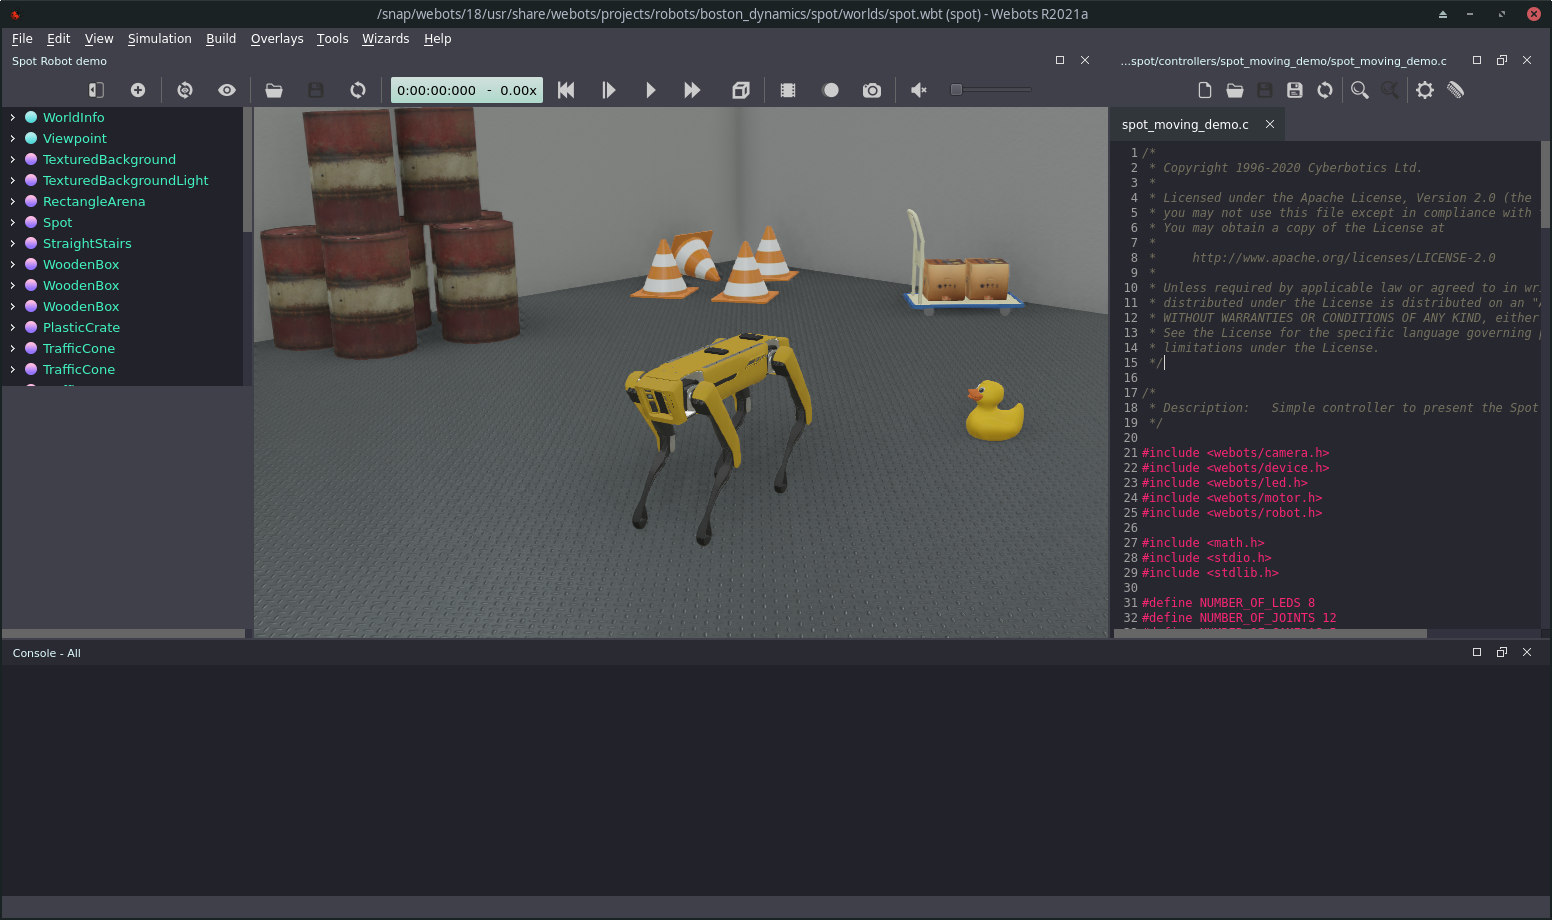
\includegraphics[width=0.85\textwidth]{webots_ide.png}
\caption{Integrirano razvojno okruženje za WebotsR2021a}
\label{fig:webots_ide}
\end{figure}

\newpage
\section{Gradivne jedinice Webots projekta}
Webots projekt sadrži se od svjetova, kontrolera (engl. \textit{controller}), robota te opcionalno, korisnički implementirane fizike. Komponente su međusobno u hijerarhijskoj ovisnosti, gdje je roditelj hijerarhije gradivna jedinica svijet. Simulacija se odvija nad jednim svijetom koji može imati više robota te svaki robot može imati više kontrolera, iako samo jedan može biti i aktivno vezan za njega. Prilikom izrade Webots projekta automatski se generira direktorijska struktura sa sljedećim direktorijima: \textit{worlds}, \textit{controllers}, \textit{protos}, \textit{plugins}.

\subsection{Gradivna jedinica Svijet}
Osnovna gradivna jedinica Webots projekta je svijet (engl. \textit{world}). Svijet sadrži opis svakog objekta, njegovu poziciju u svijetu te svojstva. Kako bi se točno znao odnos između objekata u svijetu svi objekti imaju svoju hijerarhiju. Primjerice ako robot sadrži senzore oni će biti enkapsulirani u objekt robota. U datoteku se svijet sprema s formatom \texttt{.wbt}. Datoteka ne sadrži implementaciju logike ponašanja objekata i njihove interakcije. Svi svjetovi korišteni u Webots projektu se nalaze u \textit{worlds} direktoriju.

\noindent{Instalacija Webots programskog paketa sadrži i razne probne (engl. \textit{demo}) svjetove koji prikazuju osnovne funkcionalnosti robota. Jedan od takvih svjetova je i \texttt{highway.wbt} koji prikazuje osnovne funkcionalnosti robota \textit{BmwX5} (Slika \ref{fig:webots_highway})}

\begin{figure}[htb!]
\centering
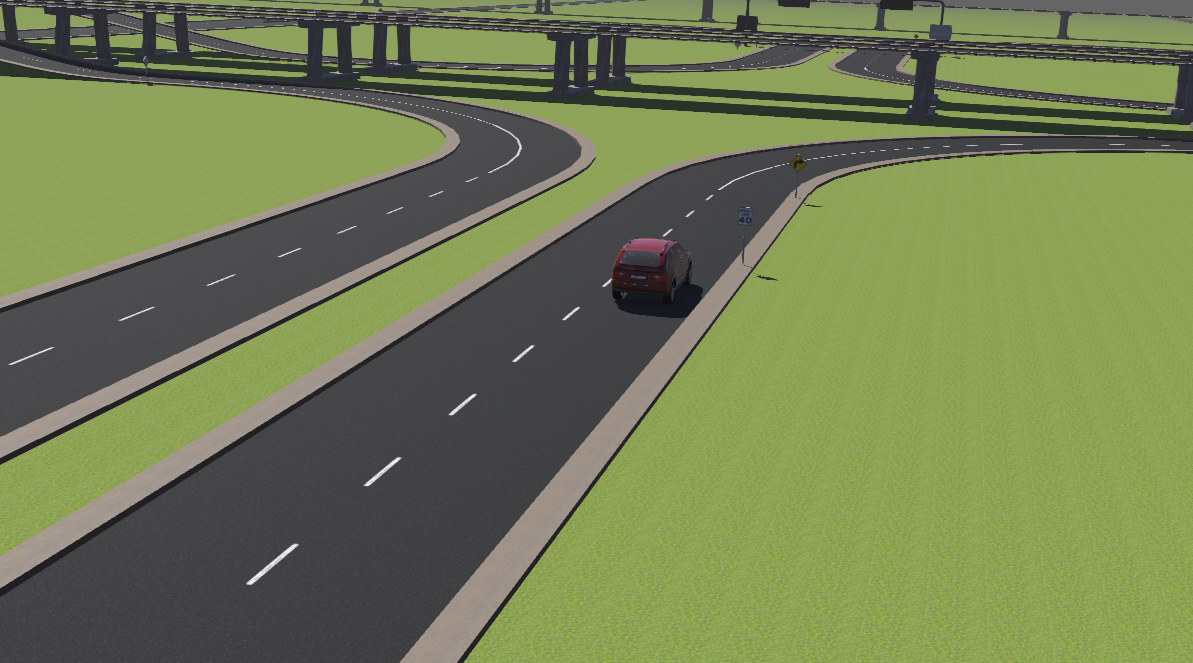
\includegraphics[width=0.75\textwidth]{webot_highway_world.png}
\caption{Prikaz svijeta highway.wbt}
\label{fig:webots_highway}
\end{figure}

\newpage
\subsection{Kontrola ponašanja objekta}
Program koji kontrolira ponašanje objekta u svijetu naziva se kontroler (engl. \textit{controller}). Kao što je već navedeno svi kontroleri sve mogu pisati u jezicima C, C++, Java i MATLAB. Učitavanjem svijeta svi kontroleri na robotima se pokreću automatski te izvršavaju simulaciju (ako kontroler nema praznu logiku). Jednom pokrenuta simulacija može se resetirati, ubrzati pauzirati ili izvoditi korak po korak. Sva ta kontrola dostupna nam je na alatnoj traci Webots integriranog razvojnog okruženja (Slika \ref{fig:webots_toolbar}).

\begin{figure}[htb!]
\centering

\includegraphics[width=0.75\textwidth]{webots_toolbar.png}
\caption{Alatna traka za kontrolu simulacije Webots svijeta}
\label{fig:webots_toolbar}
\end{figure}

\newpage
\noindent{\textit{"Hello, world!"} tip programa\footnote{"Hello, world" je najosnovniji tip programa, u određenom programskom jeziku, s kojem se novacima u programiranju pokazuje najjednostavniji mogući izvorni kod čiji izvršni kod ispisuje tekst "Zdravo, svijete!" \textit{"Hello, world!"} na standardni izlaz.} za Webots kontroler mogao bi izgledati na sljedeći način.}

\begin{minted}[linenos, frame=lines, fontsize=\small]{cpp}
#include <webots/Robot.hpp>
#include <iostream>

int main()
{
  webots::Robot *robot = new webots::Robot();
  while (robot->step(32) != -1)
    std::cout << "Ah, ha, ha, ha, stayin' alive" << std::endl;
  delete robot;
  return 0;
}
\end{minted}

\noindent{Osim naravno uključivanja svih potrebnih biblioteka u program, najbitnije nam je inicijalizirati objekt klase \texttt{Robot} i koristiti njezinu virtualnu funkciju \texttt{robot->step(mi\-lliseconds)}. Poziv funkcije \texttt{robot->step(32)} u našem kodu računa stanje simulacije 32 milisekunde u budućnost simuliranog vremena. Moramo primijetiti kako se simulirano vrijeme razlikuje od stvarnog vremena što nam omogućava točnost simulacije na računalima različitih performansi. Može se dogoditi ako imamo dovoljno kompleksnu scenu da se onda izgenerira tek nakon pet sekundi bez obzira na to što je prošlo 32 milisekunde simulacije.}

\noindent{Povratna vrijednost funkcije \texttt{robot->step()} je -1 ako se prekida rad kontrolera što se može dogoditi zbog restartanja simulacije svijeta, gašenjem Webots programa, učitavanjem novog svijeta, itd. U našem primjeru programski isječak unutar \texttt{while} petlje će se ponavljati u beskonačnost sve dok ga ručno ne ugasimo.}

\noindent{Kontroler ne može direktno manipulirati tijekom simulacije (pauzirati, zaustavljati, ponovno pokretati). U tu svrhu uvodi se gradivna jedinica \textit{Supervisor}. Ona nije korištena u ovoj implementaciji, ali bi se mogla koristiti primjerice u svrhu implementacije podržanog učenja kretnje bipedalnog modela.}

\subsection{Gradivna jedinica Robot}
Modeli čija ponašanja programiramo u Webots svijetu su roboti. Webots programski paket podržava veliku listu modela robota iz stvarnog svijeta te stvaranje vlastitih modela robota. Kako se Webots često koristi u svrhe simuliranja, njegova svrha može biti veoma korisna prije stvaranja modela u stvarnome svijetu. Zbog toga, Webots sadrži razne modele poznatih robota kao što su četveronožni \textit{Spot} i dvonožni \textit{Atlas} (Slika \ref{fig:atlas}) tvrtke \textit{Boston Dynamics}.

\noindent{Osim njih na listi\footnote{https://cyberbotics.com/doc/guide/robots} se mogu pronaći robota tvrtki Sony, Sphero, Fujitsu, DJI, itd. Svi navedeni modeli dozvoljeni su za besplatno korištenje pod \textit{Cyberbotics} licencom\footnote{https://cyberbotics.com/webots\_assets\_license}.}

\noindent{Roboti na sebi mogu sadržavati razne senzore čiji se podaci mogu koristiti za implementaciju različitih funkcionalnosti. Senzori koje podržava programski paket Webots su: kamere, senzor udaljenosti, lidar te radar.}

\begin{figure}[htb!]
\centering
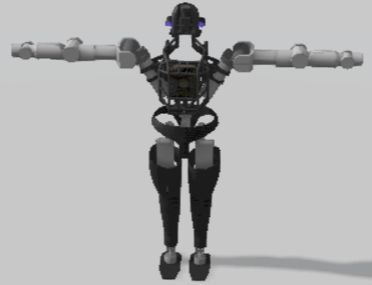
\includegraphics[width=0.70\textwidth]{atlas.png}
\caption{3D model robota Atlas u programskog paektu Webots}
\label{fig:atlas}
\end{figure}

\newpage
\section{Simulacija Webots svijeta u web-pregledniku}
Vrlo zgodna funkcionalnost Webotsa je što nam omogućava generiranje scene i animacije svijeta za web-preglednik (engl. \textit{web browser}).

\noindent{Web scena nam omogućava kretanje po svijetu te ručno pomicanje objekata, ako nam je to omogućeno. Scena ne sadrži informacije i simulaciji i kontrolere tako da se one koriste za prezentaciju statičnih objekata.}

\noindent{Web animacija nam omogućava reproduciranje interaktivnog videa Webots svijeta. Animacija se može izraditi snimanjem određenog djela simulacije koje se onda reproducira u web-pregledniku. Prilikom reprodukcije moguće je kretati se kamerom u prostoru svijeta te je pauzirati i premotavati. (Slika \ref{fig:webots_webgl})}

\noindent{Nažalost zbog korištene knjižnice \textit{three.js} temeljene na grafičkoj knjižnici WebGL, reprodukcije animacije u web-pregledniku se ne mogu pokretati u \textit{Google Chrome} web-pregledniku\footnote{https://cyberbotics.com/doc/guide/web-scene\#remarks-on-the-used-technologies-and-their-limitations (lipanj, 2021.)}. }

\begin{figure}[htb!]
\centering
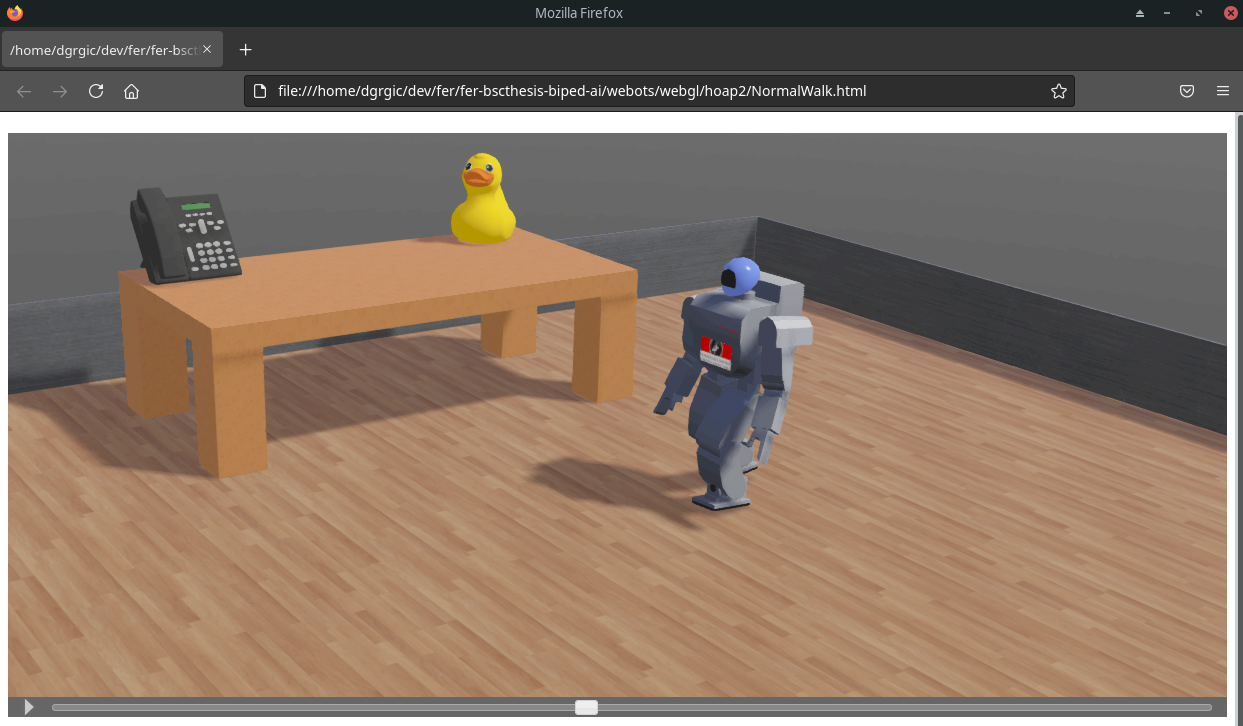
\includegraphics[width=0.85\textwidth]{webot_webgl.png}
\caption{Prikaz simulacije Webots svijeta u Firefox web-pregledniku}
\label{fig:webots_webgl}
\end{figure}

\chapter{Umjetne neuronske mreže}
Jedno od najznačajnijih grana računalne znanosti danas je umjetna inteligencija čija popularnost neupitno raste godinama. Dokaz tome je popularizacija servisa u obliku (engl. \textit{cloud service}) čija svrha je dozvoliti pristup istraživačima rad na snažnim jedinicama napravljenim isključivo za obradu problema umjetne inteligencije. Jedan od takvih servisa je \textit{Google Colaboratory}\footnote{https://research.google.com/colaboratory/} koji omogućava besplatno (na određen broj ciklusa) ili uz vrlo malu nadoplatu korištenje tenzorskih procesorskih jedinica (engl. \textit{tensor procesor unit} - TPU)\footnote{https://cloud.google.com/tpu}. Na ovaj način istraživači mogu procesirati kompleksne algoritme čije bi vrijeme izvršavanja bilo znatno veće na njihovim osobnim računalima.

\noindent{Mogući pristup problemima umjetne inteligencije su umjetne neuronske mreže. Neuronske mreže\footnote{U nastavku rada koristit ćemo naziv neuronske mreže za umjetne neuronske mreže bez gubitka značenja.} su sustavi temeljeni na biološkim neurološkim sustavima u tijelu čovjeka koji rješavaju probleme klasifikacije i funkcijske regresije.}

\noindent{Klasifikacija je postupak svrstavanja ulaznih uzoraka u razrede, a funkcijska regresija je postupak aproksimacije funkcije na ulaznim podacima (\cite{cupic2018unm}).}

\noindent{Snaga bioloških neurona (živčanih stanica) motivacija je za nastajanje umjetnih neurona kao računalne strukture koja omogućava drugačiji pristup računalno zahtjevnim problemima.}

\noindent

\newpage
\section{Struktura umjetnog neurona}
Gradivna jedinica neuronske mreže je umjetni  neuron (Slika \ref{fig:artifical_neuron}). Njegova građa temelji se na biološkom neuronu (Slika \ref{fig:biological_neuron}) te se na takav način veže s ostalim neuronima u mreži.

\begin{figure}[htb!]
\centering
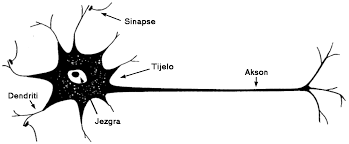
\includegraphics[width=0.75\textwidth]{biological_neuron.png}
\caption{Biološki neuron (izvor: hrcak.srce.hr)}
\label{fig:biological_neuron}
\end{figure}

\begin{figure}[htb!]
\centering
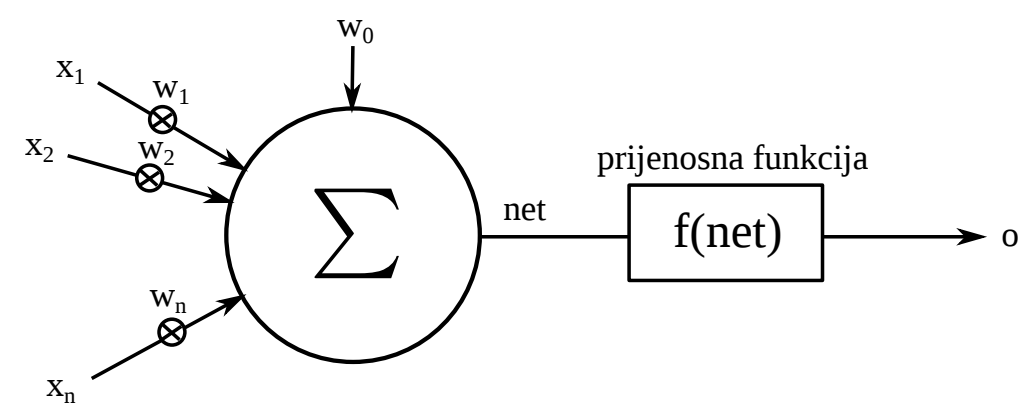
\includegraphics[width=0.75\textwidth]{aritifical_neuron.png}
\caption{Umjetni neuron u strukturi neuronske mreže (izvor: \cite{cupic2018unm})}
\label{fig:artifical_neuron}
\end{figure}

\noindent{Možemo primijetiti da se ulazi u mrežu $x_{1}, x_{2}, \dots, x_{n}$ ponašaju poput dendrita biološkog neurona. Ulazi $x_{1}, x_{2}, \dots, x_{n}$ množe se s težinom na svakom ulazu $w_{1}, w_{2}, \dots, w_{n}$. Prolaskom kroz čvor sa znakom sume na slici tj. funkciju net dobijemo vrijednost zadanu idućom formulom:}
\begin{equation} \label{eq:net_calculate}
net = \sum_{i=1}^{n} x_{i} * w_{i} + w_{0}
\end{equation}

\noindent{Nakon izračunavanja $net$ vrijednosti računa se vrijednost prijenosne funkcije $f(net)$. Postoje razne prijenosne funkcije: sigmoidalna, funkcija skoka, funkcija identiteta, tangens hiperbolni, zglobnica (nepropusna i propusna), itd. U svrhu izrade ovoga rada korištene su sigmoidalna funkcija i tangens hiperbolni (Slika \ref{fig:artifical_func}).}

\noindent{Jedan od poznatijih umjetnih neurona je TLU-perceptron (engl. \textit{Treshold Logic Unit} čija je prijenosna funkcija funkcija skoka (\cite{mcculloch43a})}

\begin{figure}[htb!]
\centering
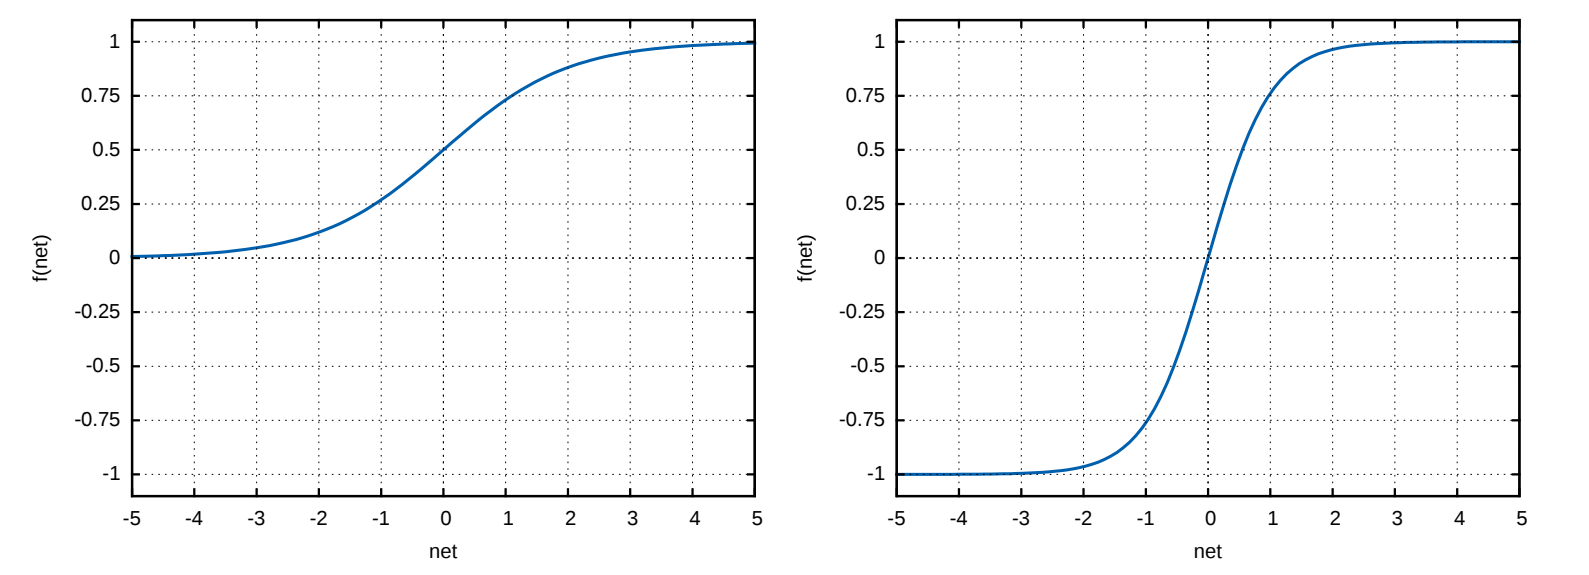
\includegraphics[width=1.0\textwidth]{aritifical_functions.png}
\caption{Sigmoidalna funkcije i tangens hiperbolni (izvor: \cite{cupic2018unm})}
\label{fig:artifical_func}
\end{figure}

\section{Struktura neuronske mreže}
Neuronske mreže se sastoje od tri djela: ulazni sloj, skriveni slojevi i izlazi sloj. Svaki sloj može imati jedan ili više neurona\footnote{U nastavku rada koristit ćemo naziv neuron za umjetni neuron bez gubitka značenja.}. Ako neuron pod rednim brojem $j$ u sloju $i$ označimo kao $y_{j}^{(i)}$ onda je neuron $y_{j}^{(i)}$ povezan sa svim neuronima u sloju $i+1$ (osim ako je $i$ izlazni sloj). Takvu strukturu grafički možemo prikazati slikom \ref{fig:artifical_neural_network}.

\begin{figure}[htb!]
\centering
\includegraphics[width=0.85\textwidth]{artifical_neural_netnjork.png}
\caption{Prikaz neuronske mreže sa dva skrivena sloja (izvor: \cite{cupic2018unm})}
\label{fig:artifical_neural_network}
\end{figure}

\noindent{Ako želimo opisati arhitekturu mreže to možemo učiniti tako da za svaki sloj napišemo broj neurona u sloju te takve brojeve povežemo u zapis znakom $\times$. Primjerice arhitektura mreže na slici \ref{fig:artifical_neural_network} tada bi bila $2\times5\times3\times2$.}

\section{Korištenje neuronskih mreža}
Korištenje neuronskih mreža se provodi u dva dijela: treniranje i predviđanje. 

\subsection{Treniranje}
U prvom koraku potrebno je vektor vrijednosti značajki iz skupa podataka propagirati kroz neuronsku mrežu unaprijed od ulaznog do izlaznog sloja. Početne vrijednosti težina postavljene su nasumično te se za svaki neuron izračuna njegova $net$ vrijednost korištenjem izraza \ref{eq:net_calculate}. To je samo jedan prolazak kroz mrežu, a učenje se zapravo odvija tako da se korištenjem algoritma unazadnog širenja (engl. \textit{backpropagation}) namještaju težine tako da se smanji greška predviđenih s obzirom na ulazne podatke. Prilikom učenja podatke dijelimo na skup za učenje i na skup za testiranje (u nekim slučajevima dodatno imamo i skup validacije). Bitno je naglasiti i da se skup podataka mora normalizirati na vrijednosti u rasponu [0, 1].

\subsubsection{Algoritam unazadnog širenja} \label{sec:backprop}
Algoritam unazadnog širenja konceptualno popravlja težine mreže tako da se smanji greška s obzirom na vrijednosti izlaznog sloja mreže. Dvije vrijednosti su nam bitne u ovom algoritmu $\delta$ i $\eta$. Grčko slovo $\delta$ nam predstavlja grešku u i-tom neuronu j-tog sloja, a $\eta$ vrijednost između 0 i 1 koju zadajemo sami. Algoritam po koracima računa: 
\begin{enumerate}
\item Izračunaj pogrešku i-tog izlaznog neurona sljedećim izrazom $\delta_{i}^{(j)} = y_{i}^{(j)} * (1 - y_{i}^{(j)} * (Y_{i}^{(j)} -y_{i}^{(j)})$ gdje $\delta_{i}^{(j)}$ predstavlja grešku i-tog neurona u j-tom sloju $y_{i}^{(j)}$ predstavlja predviđenu vrijednost u neuronu, $Y_{i}^{(j)}$ predstavlja stvarnu vrijednost. 
\item Sada se od izlaznog sloja krećemo prema ulaznom sloju mreže te u ovom slučaju grešku računamo izrazom $\delta_{i}^{(j)} = y_{i}^{(j)} * (1 - y_{i}^{(j)})* \sum_{d}(\delta_{d}^{(j+1)} * f'(w))$ gdje $f'(w)$ predstavlja derivaciju prijenosne funkcije, a  $\delta_{d}^{(j+1)}$ greške sloja $j+1$ koji su povezani s neuronom $i$.
\item Težinu za svaki neuron korigiramo izrazom $w_{i}^{(j)} = w_{i}^{(j)} + \eta * y_{i}^{(j)} * \delta_{i}^{(j)}$.
\end{enumerate}

\noindent{Za svaki ulaz u skupu podataka za treniranje odrađujemo ovaj algoritam dok se greška ne smanji na željenu vrijednost ili sami prekinemo učenje.}

\subsection{Predviđanje} 
Jednom takvu utreniranu mrežu ubacujemo svoje podatke te vršimo propagaciju unaprijed. Takve izlaze koristimo kao podatke u postupcima funkcijske regresije ili klasifikacije. Bitno je samo da prije korištenja podataka invertiramo normalizaciju tako da nam vrijednosti poprimaju raspone domene kakva je bila u ulaznome skupu.

\section{Funkcijske knjižnice za implementaciju neuronskih mreža}
U svrhu izrade modela u ovome radu korištene su programske knjižnice za izradu neuronskih mreža Sklearn (\cite{scikit-learn}) i Keras(\cite{chollet2015keras}). Ove dvije biblioteke omogućavaju brzu implementaciju neuronske mreže, njezino korištenje te spremanje i učitavanje već utreniranih modela u programskom jeziku Python. 

\noindent{Stvoriti mrežu sa slike \ref{fig:artifical_neural_network} putem ovih programskih knjižnica možemo napraviti idućim izvornim kodom:}
\begin{minted}[linenos, frame=lines, fontsize=\small]{py}
model = Sequential([
    Dense(2),
    Activation('sigmoid'),
    Dense(5),
    Activation('sigmoid'),
    Dense(3),
    Activation('sigmoid'),
    Dense(2)
])
\end{minted}
\noindent{U ovome programskom isječku objekt \texttt{Dense} predstavlja obični sloj neuronske mreže povezan kao na slici \ref{fig:artifical_neural_network}}. U njegov konstruktor navodimo broj neurona u sloju. Između svakog sloja definiramo prijenosnu funkciju za neurone tog sloja korištenjem objekta \texttt{Activation}. Taj objekt u svoj konstruktor prima tip prijenosne funkcije, u našem slučaju to je sigmoidalna funkcija.

\noindent{Objekt \texttt{model} koji smo stvorili možemo koristiti pozivajući funkcije \texttt{model.fit()} i \texttt{model.predict()}. Osim osnovnih funkcionalnosti funkcijska knjižnica Keras omogućava nam funkcionalnosti poput automatskog zaustavljanja učenja nakon određene minimalne pogreške te pozivanje korisničke funkcije prilikom ostvarivanja događaja (engl. \textit{callback functions})}. 

\noindent{Isto tako možemo definirati maksimalan broj epoha tj. broj ponavljanja po skupu podataka za treniranje prije prestanka učenja. Prema predodređenim postavkama model će podijeliti skup na skup za treniranje i skup za testiranje u postotcima 70\% i 30\%.}

\chapter{Implementacija}
U svrhu implementacije kontrole ponašanja robota korišten je programski jezik C++ i programski paket Webots, a za generiranje modela neuronskih mreža, crtanje grafova i generiranje novih podataka korišten je programski jezik Python i već navedene knjižnice Sklearn i Keras.

\section{Model robota}
Robot Fujitsu HOAP2 (engl. \textit{Humanoid for Open Architecture Platform}) je model čovjekolikog robota visine 48 cm s 25 stupnjeva slobode (Slika \ref{fig:hoap2}). Detaljan popis zglobova nalazi se u Dodatku \ref{sec:fujitsu_hoap2}. Svaki zglob u 3D prostoru ima mogućih 6 stupnjeva slobode a to su: translacija u svakoj od tri koordinate prostora te rotacija u svakoj od tri koordinate prostora. U Webots modelima svaki stupanj slobode za određeni zglob ima svoju vrijednost u dvostrukoj preciznosti koju možemo postaviti.

\begin{figure}[htb!]
\centering
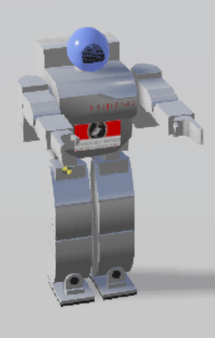
\includegraphics[height=0.42\textwidth]{hoap2.png}
\caption{Fujitsu HOAP2}
\label{fig:hoap2}
\end{figure}

\newpage
\section{Hod robota}
Sve kretnje robota osnivaju se na slijedu točno određenih stupnjeva rotacija zglobova u svakom trenutku simulacije. U našem slučaju od svih dostupnih zglobova (Dodatak \ref{sec:fujitsu_hoap2}), korišteni su samo: dva stupnja slobode oba ramena, jedan stupanj slobode oba kuka, oba koljena i oba gležnja.

\noindent{Kretanje je napravljeno periodički. Ako napravimo graf ovisnosti kutu rotacije zgloba i vremenu možemo primijetiti da se vrijednosti rotacije kuka ponavljaju nakon iskoraka lijevom i iskoraka jednom nogom. Na slici \ref{fig:leg_angles} možemo vidjeti ovisnost kuta zglobova noge kroz vrijeme simulacije. Značenje negativnog kuta na grafu govori da je zglob otklonjen u suprotni smjer od početne pozicije. Isti kut sa suprotnim predznakom daje otklonjenost u suprotnoj orijentaciji.}

\begin{figure}[htb!]
\centering
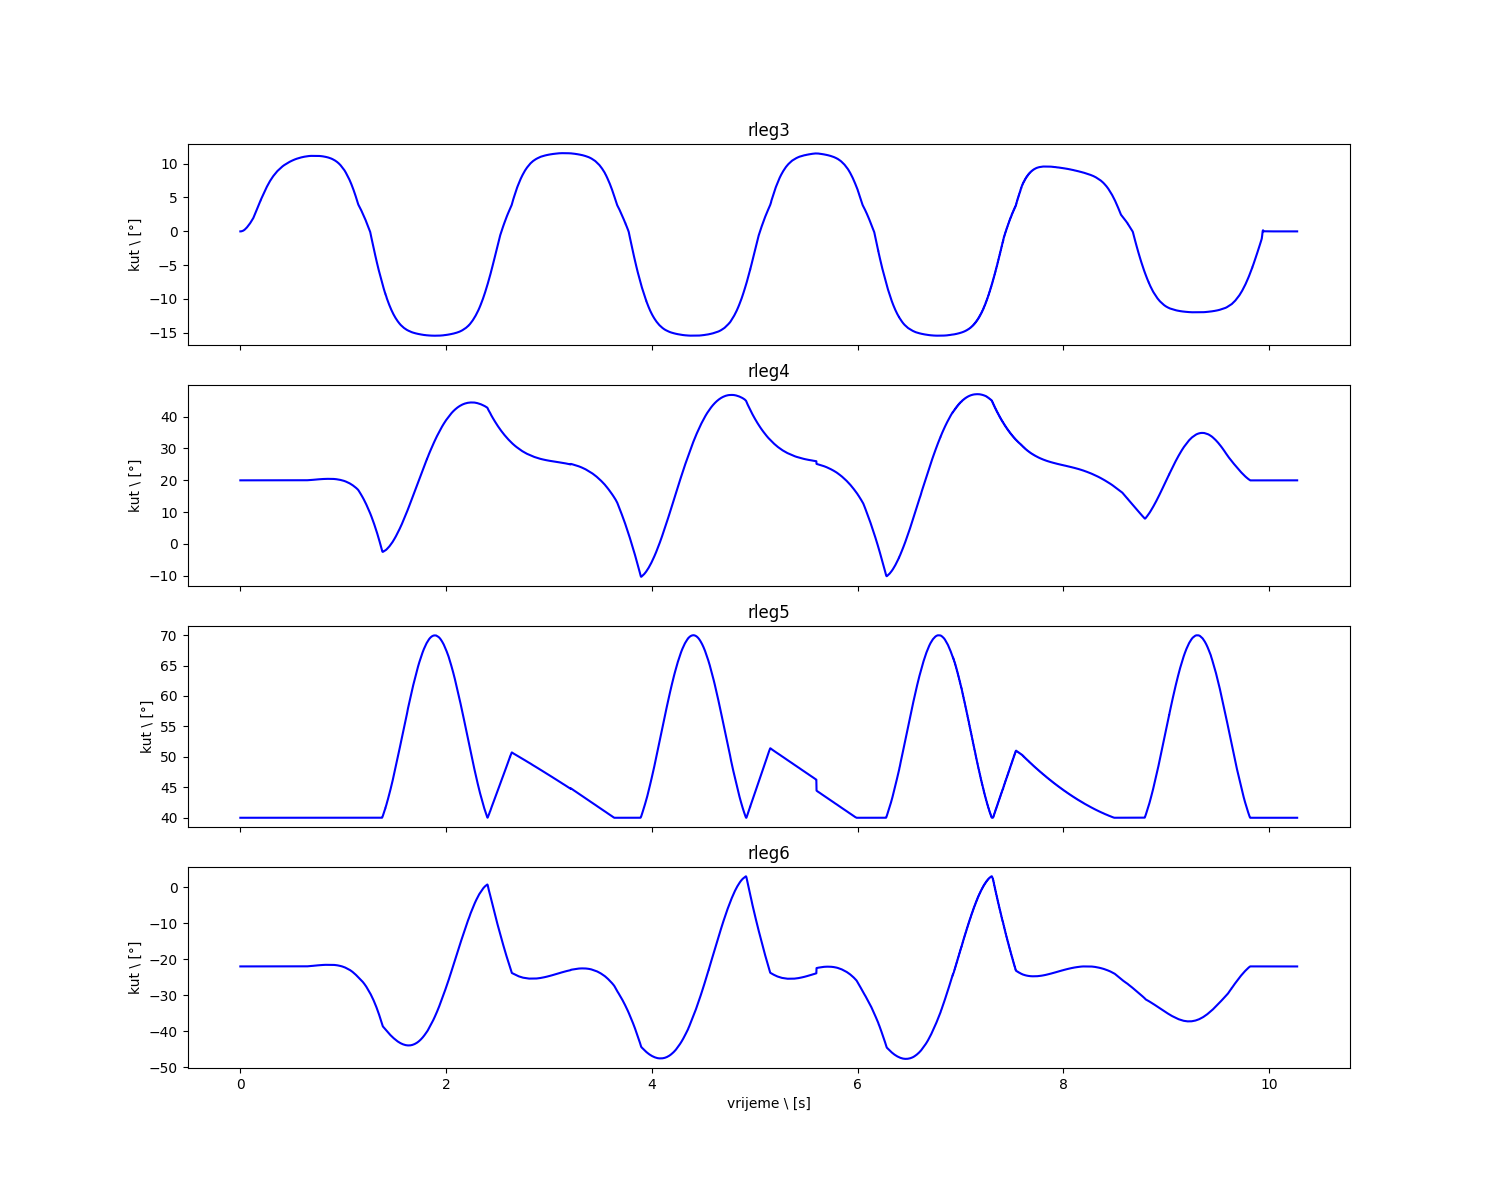
\includegraphics[width=1.0\textwidth]{anglesLeg.png}
\caption{Graf ovisnosti kuta zgloba kroz vrijeme simulacije.}
\label{fig:leg_angles}
\end{figure}

\noindent{Prvi graf predstavlja jedan kut slobode kuka te vidimo funkciju sličnu sinusoidalnoj funkciji. Na početku i kraju vidimo razliku kako je hod sporiji zbog kretanja i stajanja. Isti takav trend možemo vidjeti na ostalim grafovima. Drugi graf prikazuje kretnje koljena, a treći i četvrti predstavljaju kretnje gležnja kroz vrijeme. Svi grafovi su jednaki za lijevu nogu samo je faza pomaknuta za duljinu jednoga koraka. To možemo vidjeti vizualno na slici \ref{fig:leg_phase}. Najbolje se trajanje koraka može primijetiti gledajući oštre špiceve crvenog grafa (lijeve noge) i plavog grafa (desne noge).}

\begin{figure}[htb!]
\centering
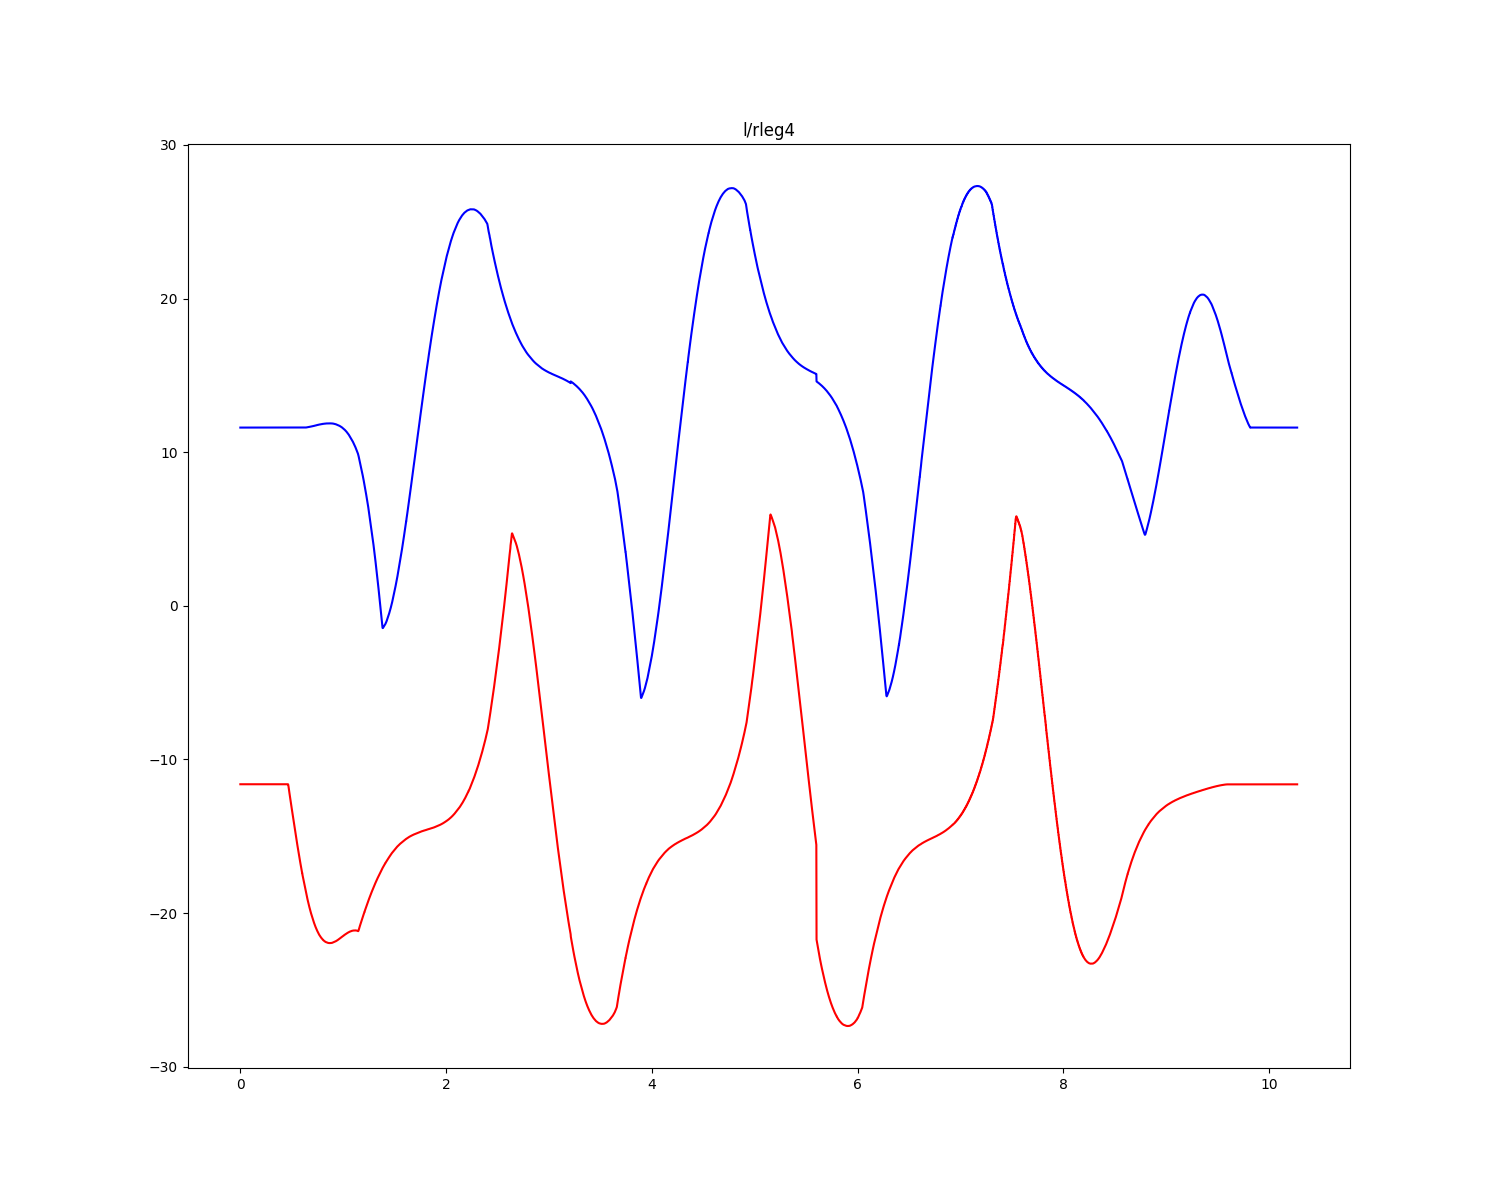
\includegraphics[height=0.75\textwidth]{anglePhase.png}
\caption{Graf ovisnosti kuta zgloba kroz vrijeme simulacije lijevog i desnog koljena.}
\label{fig:leg_phase}
\end{figure}

\subsection{Generiranje i učitavanje datoteke s kretnjama}
Zbog mogućnosti grafova koje nas navodi na rješavanja problema učenja funkcijskom regresijom, idući prirodni korak je generirati datoteke s podacima o kutovima zglobova kroz vrijeme. Najzgodniji format u te svrhu je CSV datoteka (engl. \textit{comma separated values}). Kreiranu kretnju sada kopiramo u CSV datoteku koja će se lako moći koristiti i u treniranju modela. Prvih 6 stupaca datoteke izgledaju na sljedeći način. Stupci tablice označeni su simboličkim nazivljem zglobova (Dodatak \ref{sec:fujitsu_hoap2}). 

\begin{filecontents*}{sample.csv}
    2,-3,993,4178,8357,-4598,1372,17090,-2091,-2090,5222,0,1483,-4180,-8360,4595,1371,-20529,2087,2087,-5228
    2,-3,993,4178,8357,-4598,1372,17090,-2091,-2090,5222,0,1483,-4180,-8360,4595,1371,-20529,2087,2087,-5228
    2,-3,1000,4178,8357,-4598,1379,17085,-2091,-2090,5222,0,1491,-4180,-8360,4595,1378,-20534,2087,2087,-5228
\end{filecontents*}

\noindent{
\begin{tabular}{lll|ll|l}%
    \bfseries rleg\_joint1 & \bfseries rleg\_joint2 & \bfseries rleg\_joint3 & \bfseries rleg\_joint4 & \bfseries rleg\_joint5 &\bfseries rleg\_joint6
    \csvreader[head to column names]{sample.csv}{}
    {\\\hline\csvcoli&\csvcolii&\csvcoliii&\csvcolvi&\csvcolv&\csvcolvi}
\end{tabular}}

\noindent{Sve varijabilne vrijednosti u tablici pomnožene su s vrijednosti 209 što je vrijednost širine pulsnog signala servo motora Fujitsu HOAP2 robota.}

\noindent{Kontroler robota sadrži učitavanje vrijednosti CSV datoteke te postavljanje vrijednosti kuta zglobova robota svakih 50 milisekundi simulacije.}

\begin{minted}[linenos, frame=lines, fontsize=\small]{cpp}
// ...
// učitaj podatke idućih pozicija iz CSV datoteke
sscanf(motion,
    "%*d, %d, %d, %d, %d ,%d, %d, %d, %d, %d,"
    " %d, %d, %d, %d, %d, %d, %d, %d, %d, %d,"
    " %d, %d",
    &posFromCsv[(int)Joints::rleg_joint_1],
    // ...
    &posFromCsv[(int)Joints::body_joint_1]);

// pretvori kutove u radijane
for (int i = 0; i < jointsNum; i++)
    nextPosition[i] = posFromCsv[i] * (M_PI / 180.0) / pulse[i];
// postavi kutove zglobova
joint[(int)Joints::body_joint_1]->setPosition(...);
// ...
\end{minted}

\noindent{Svi servo motori sadrže svoju enumeraciju kako bi im se moglo lakše pristupiti te se pozicija kuta motora u radijanima postavlja naredbom \texttt{join->setPosition(angle)}.}

\newpage
\section{Neuronske mreže za funkcijsku regresiju}
Analizom grafova funkcija, zaključak je da je potrebno napraviti dvije neuronske mreže koje će se trenirati za svaki pojedinačni zglob. Jedna neuronska mreža će trenirati "špicaste" sinusoidne funkcije (iscrtane crveno na slici \ref{fig:func_types}), dok će druga trenirati "glatke" sinusoidne funkcije s brjegovima i dolovima (iscrtane plavo na slici \ref{fig:func_types}). Takav pristup dao je najbolje ishode učenja i predviđanja vrijednosti.

\begin{figure}[htb!]
\centering
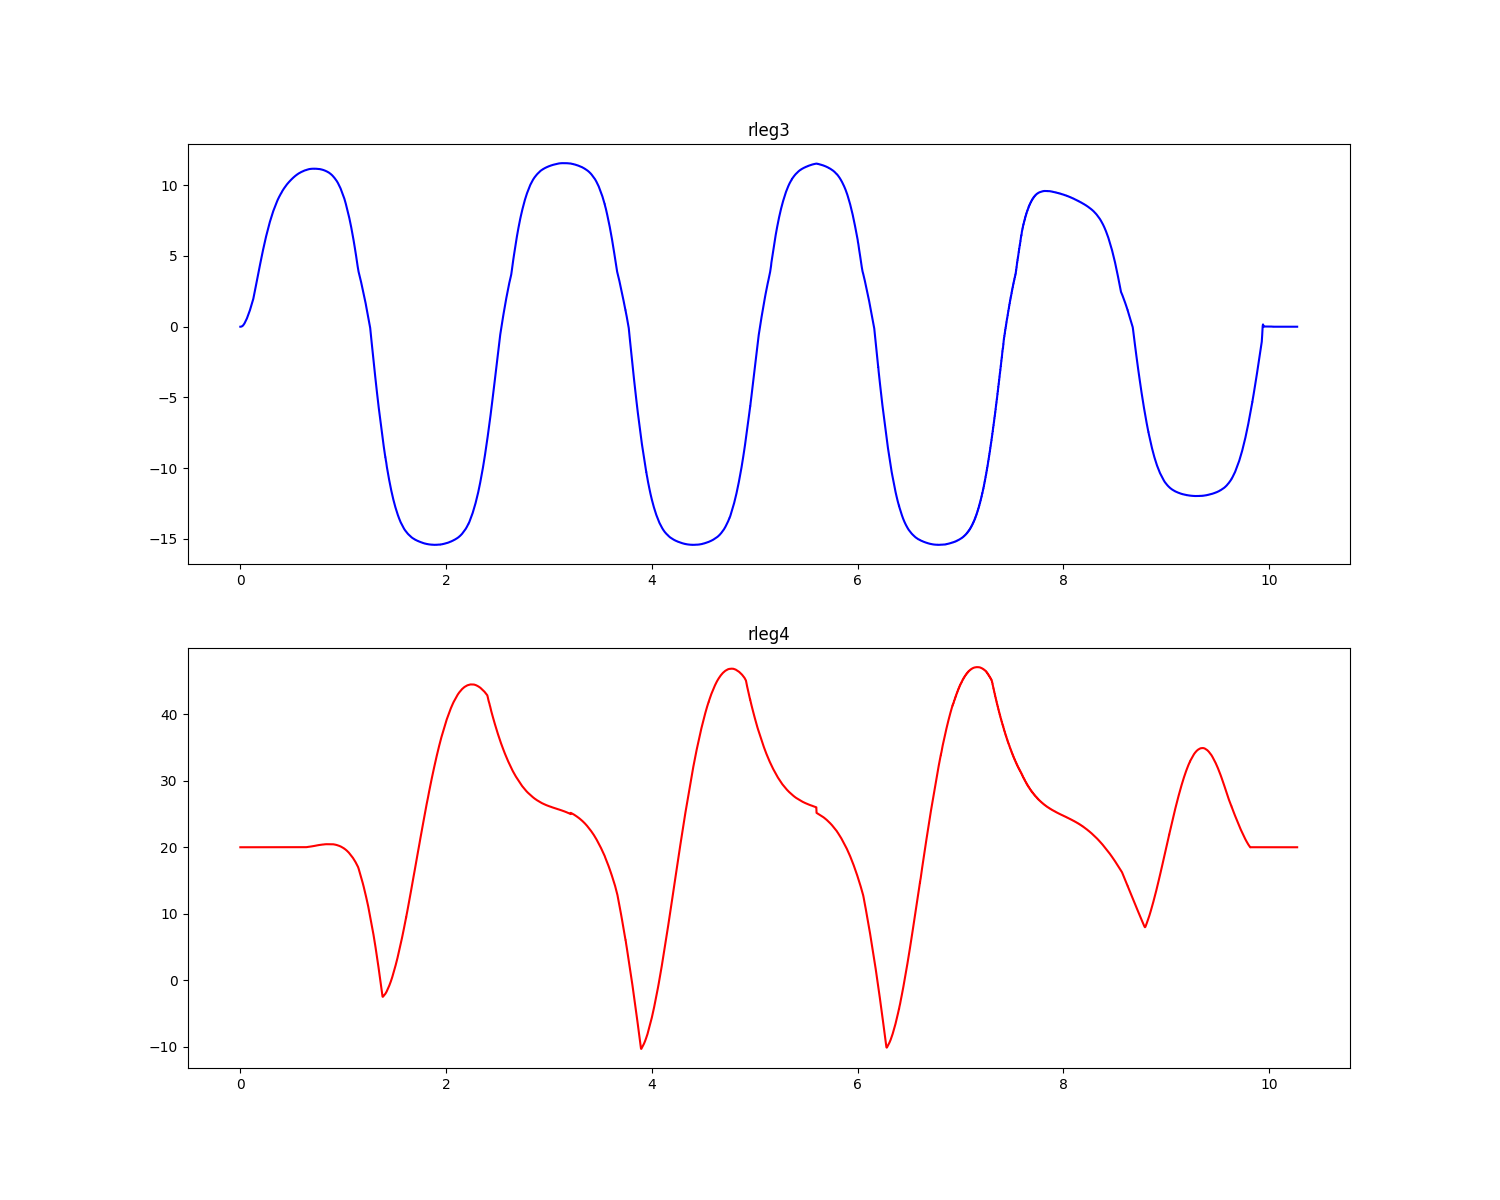
\includegraphics[height=0.75\textwidth]{functionTypes.png}
\caption{Dva tipa funkcija za koje su namijenjene neuronske mreže.}
\label{fig:func_types}
\end{figure}

\noindent{Prilikom treniranja za vrijednost greške koristi se RMSE (engl. \textit{root mean squared error}) vrijednosti koja se računa računajući standardnu devijaciju pogreške svih neurona u slojevima. Pogreška neurona u sloju računa se tijekom provođenja algoritma širenja unazad (Poglavlje \ref{sec:backprop}).}

\newpage
\subsection{Neuronska mreža za "glatke" sinusoidne funkcije}
Arhitektura neuronske mreže za "glatke" sinusoidne funkcije je $150\times50\times25\times1$ što znači da sadrži ulazni sloj veličine 150, dva skrivena sloja veličina 50 i 25 te izlazni sloj veličine 1. Prijenosne funkcije u svim neuronima su sigmoidalne funkcije. Model s mješavinom tangens hiperbolne prijenosne funkcije u svim slojevima osim u izlaznom je u slučaju ovoga rada dao je veoma slične.

\subsection{Neuronska mreža za "špicaste" sinusoidne funkcije}
Arhitektura neuronske mreže za "špicaste" sinusoidne funkcije je $150\times50\times25\times25\times1$ što znači da sadrži ulazni sloj veličine 150, tri skrivena sloja veličina 50, 25 i 25 te izlazni sloj veličine 1. Prijenosne funkcije u svim neuronima su sigmoidalne funkcije. Model s mješavinom tangens hiperbolne prijenosne funkcije u svim slojevima osim u izlaznom je u slučaju ovoga rada dao je puno lošije rezultate. Isto tako bilo koja promjena broja neurona u skrivenih slojeva bi veličinu RMSE greške povećala s vrijednosti $10^{-4}$ na $10^{-2}$.

\subsection{Proces treniranja}
Obe neuronske mreže trenirane su 500 epoha na svojim odgovarajućim skupovima podataka za pojedinačni zglob. Svakih 50 epoha iskorištena je povratna funkcija za spremanje modela u datoteku. Sljedeći programski isječak korišten je u treniranju oba modela.

\begin{minted}[linenos, frame=lines, fontsize=\small]{python}
# normalizacija vrijednosti
x = asarray([i for i in range(0,len(arr))])
y = asarray(arr)

x = x.reshape((len(x), 1))
y = y.reshape((len(y), 1))

scale_x = MinMaxScaler()
x = scale_x.fit_transform(x)
scale_y = MinMaxScaler()
y = scale_y.fit_transform(y)

# treniranje modela
filepath = "models/" + joint + "/saved-model"
checkpoint = ModelCheckpoint(filepath, monitor='loss, mode='min',
    verbose=1, save_best_only=False, save_weights_only=False)
history = model.fit(x, y, epochs=500, 
    batch_size=10, verbose=2, callbacks=[checkpoint])
\end{minted}

\noindent{Jednom istrenirani model možemo učitati kada nam je potreban te pozvati funkciju \textittt{model.predict()} kako bi dobili predviđene vrijednosti funkcijske regresije. Taj postupak radimo kada generiramo CSV datoteku koja se učitava prilikom izvršavanja simulacije.}

\begin{minted}[linenos, frame=lines, fontsize=\small]{python}
# normalizacija vrijednosti
for joint in joints:
    path = f'models/{joint}/saved-model'
    model_load = load_model(path)
    # ...
    ywhat = model_load.predict(x)
    yhat_plot = scale_y.inverse_transform(ywhat)
    data[joint] = [int(i[0]) for i in yhat_plot.tolist()]

# spremanje dobivenih vrijednosti u .csv datoteku
f = open(f"../data/hoap2/{TITLE}_best.csv", "w")
    for i in range(0, len(body_angle)):
        row = []
        for joint in csv_header:
            row.append(str(data[joint][i]))
        f.write(','.join(row))
        f.write('\n')
    f.close()
\end{minted}

\noindent{Osim spremanja modela nakon određenih broja epoha, moguće je i spremiti najbolji model čija je vrijednost greške najmanja. Tada je samo bitno prilagoditi funkciju \textitt{model.fit()} da sprema model sa najmanjom RMSE vrijednosti.}
\newpage
\begin{minted}[linenos, frame=lines, fontsize=\small]{python}
# treniranje modela
filepath = "models/" + joint + "/saved-model" 
checkpoint= ModelCheckpoint(filepath, monitor='loss', mode='min', 
    verbose=1, save_best_only=True, save_weights_only=False)
earlyStopping = EarlyStopping(monitor='loss', 
    patience=100, mode='min')
model.compile(loss='mse', optimizer='adam')
history = model.fit(x, y, epochs=500, batch_size=10, 
    verbose=2, callbacks=[checkpoint, earlyStopping])

\end{minted}

\chapter{Rezultati}
Najbolji rezultat dao nam je hod Fujitsu HOAP2 modela koji napravi pet koraka prije nego što izgubi ravnotežu i padne. Razlog tome je dio funkcije koji obavlja zaustavljanje modela nakon hoda. Kako taj dio prilikom učenja najčešće najviše odstupa od ostalih dijelova funkcije, to se drastično može primijetiti na simulaciji hoda. 
\noindent{Modeli neuronskih mreža su vraćale vrijednost greške u rasponu $[10^{-4}-10^{-5}]$. Iako je to vrlo mala greška ona u kritičnoj fazi hoda kada je model van ravnoteže može rezultirati padom modela na pod. Slike \ref{fig:ramr1}} - \ref{fig:rleg4} prikazuju graf funkcije ovisnosti kuta o vremenu simulacije obojan plavom bojom, a graf dobiven funkcijskom regresijom crvenom bojom.

\begin{figure}[htb!]
\centering
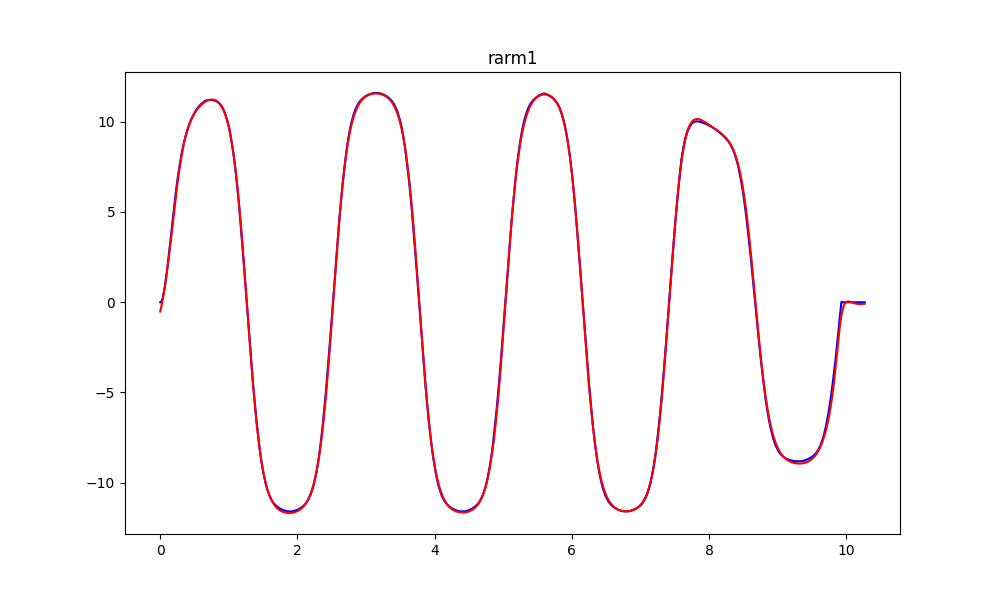
\includegraphics[width=0.75\textwidth]{rarm1.png}
\caption{Model "glatke" sinusoidne funkcije - desno rame.}
\label{fig:ramr1}
\end{figure}

\begin{figure}[htb!]
\centering
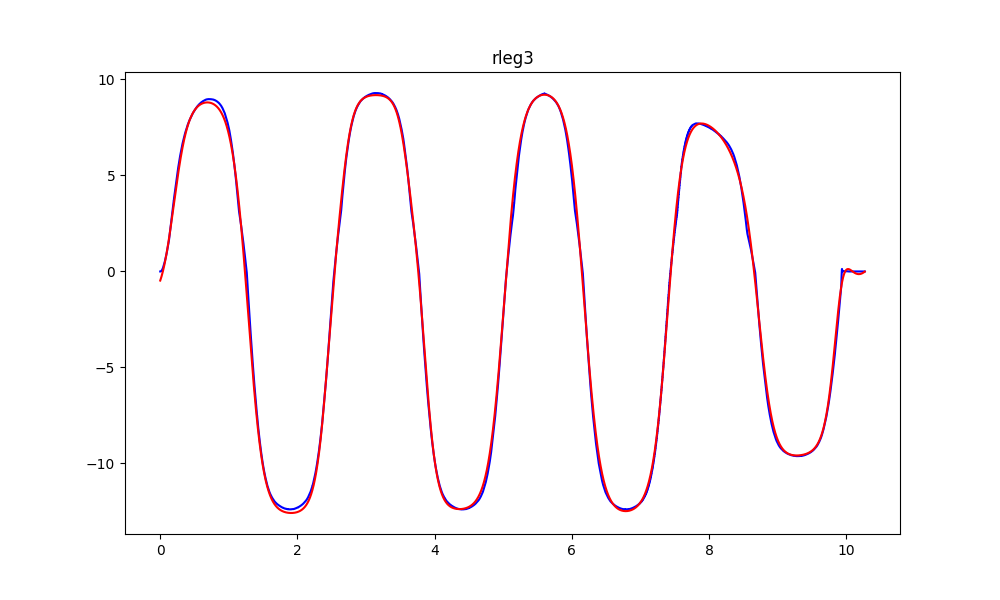
\includegraphics[width=0.75\textwidth]{rleg3.png}
\caption{Model "glatke" sinusoidne funkcije - desni kuk.}
\label{fig:rleg3}
\end{figure}

\begin{figure}[htb!]
\centering
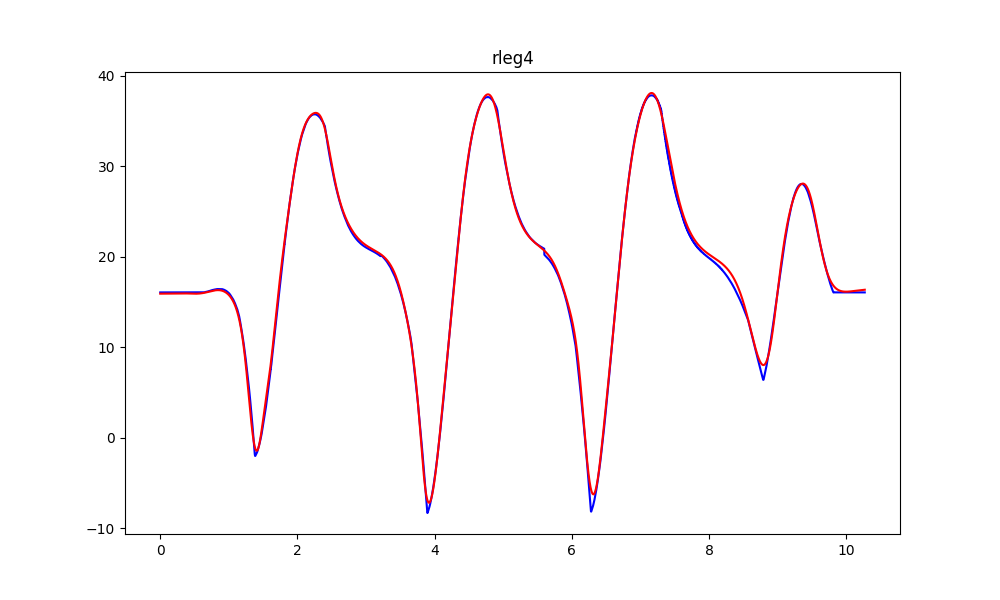
\includegraphics[width=0.75\textwidth]{rleg4.png}
\caption{Model "špicaste" sinusoidne funkcije - desno koljeno.}
\label{fig:rleg4}
\end{figure}

\begin{figure}[htb!]
\centering
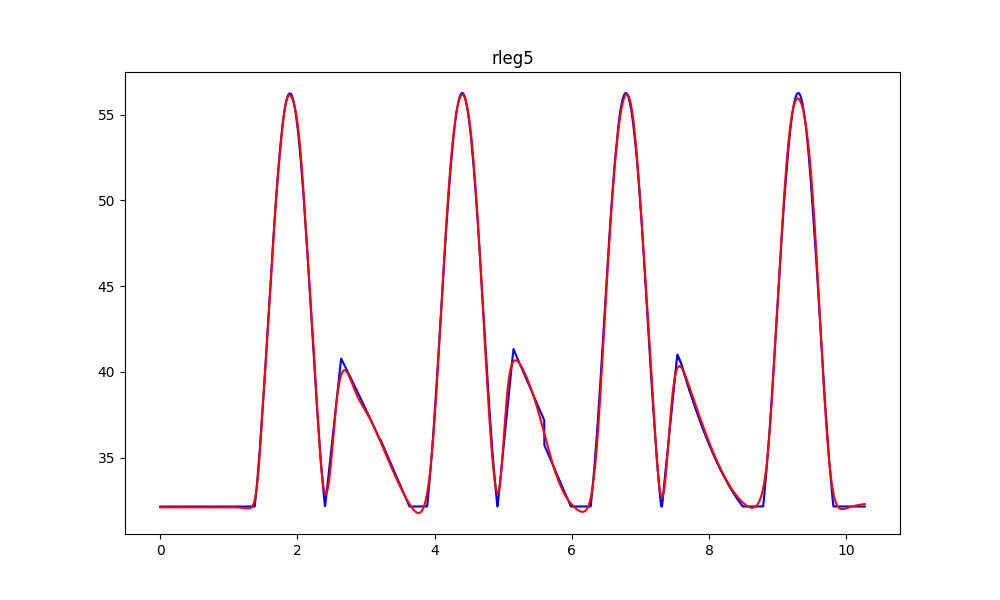
\includegraphics[width=0.75\textwidth]{rleg5.png}
\caption{Model "špicaste" sinusoidne funkcije - desni gležanj.}
\label{fig:rleg5}
\end{figure}

\noindent{Sav izvorni kod, resursi i podaci javno su dostupni na GitLab repozitoriju\footnote{https://gitlab.com/dinogrgic1/fer-bscthesis-biped-ai}}


\chapter{Zaključak}
Simulacija bipedalnog modela je vrlo složen proces koji sadrži skup raznih interdisciplinarnih znanja od fiziologije čovjeka do robotike i mehanike. Pristup rješavanja učenja hoda bipedalnog modela funkcijskom regresijom daje nam dobre rezultate za ravni teren i kratak hod.

\noindent{Bilo koja promjena terena utjecat će kobno na naš model. Zbog toga postoji mogućnost poboljšanja modela. Funkcijska regresija s običnim neuronskim mrežama funkcionira dobro na malim domenama. Bolje rezultate bi dao model LSTM koji se temeljni na konvolucijskim neuralnim mrežama. Njegova aproksimacija funkcije bila bi točnija za veće domene te bi bila brža.}

\noindent{Jedno moguće poboljšanje bez uvođenja naprednijih neuronskih mreža je smanjivanje skupa podataka na kraće cikluse tijekom hoda. Ovaj način omogućio bi nam ponavljanje ciklusa tijekom cjelokupnog hoda, a naša obična neuronska mreža bi dala bolje rezultate na još manje domene.}

\noindent{Isto tako moguće je uz pomoć Webots gradivnog objekta \textit{Supervisor} imati konstantnu kontrolu nad simulacijom te obavljati podržano učenje dinamički tijekom izvođenja simulacije što bi omogućilo "spašavanje" robota od sada neizbježnog pada.}

\chapter{Dodatak}
\section{Zglobovi Fujitsu HOAP2 robota} \label{sec:fujitsu_hoap2}
\small
\begin{itemize}
\item glava (\texttt{head\_joint[1,2}) - 2 stupnja slobode
\item tijelo (\texttt{body\_joint\_1}) - 1 stupanj slobode

\item ramena
\begin{itemize}
\item lijevo rame(\texttt{larm\_joint[1,2,3])} - 3 stupnja slobode	
\item desno rame(\texttt{rarm\_joint[1,2,3])} - 3 stupnja slobode	
\end{itemize} 

\item laktovi
\begin{itemize}
    \item lijevi lakat(\texttt{larm\_joint\_3)} - 1 stupanj slobode
    \item desni lakat(\texttt{rarm\_joint\_3)} - 1 stupanj slobode
\end{itemize}

\item zapešća
\begin{itemize}
    \item lijevo zapešće(\texttt{larm\_joint\_4)} - 1 stupanj slobode
    \item desno zapešće(\texttt{rarm\_joint\_4)} - 1 stupanj slobode
\end{itemize}

\item kuk
\begin{itemize}
    \item lijevi kuk(\texttt{lleg\_joint\_[1,2,3])} - 3 stupanja slobode
    \item desni kuk(\texttt{rleg\_joint\_[1,2,3])} - 3 stupanja slobode
\end{itemize}

\item koljeno
\begin{itemize}
    \item lijevo koljeno(\texttt{lleg\_joint\_4)} - 1 stupanj slobode
    \item desno koljeno(\texttt{rleg\_joint\_4)} - 1 stupanj slobode
\end{itemize}

\item gležanj
\begin{itemize}
    \item lijevi gležanj(\texttt{lleg\_joint\_[5,6])} - 2 stupnja slobode
    \item desni gležanj(\texttt{rleg\_joint\_[5,6])} - 2 stupnja slobode
\end{itemize}
\end{itemize}


% == literatura == 
\bibliography{literatura}
\bibliographystyle{fer}

% == sazetak -- hr == 
\newpage

\begin{sazetak}
Ovaj završni rad implementira učenje hodanja bipedalnog modela uz pomoć neuronskih mreža. Modeli robota i simulacija hoda odrađena je uz pomoć programskog paketa za simulaciju robota Webots. Učenje hoda izvršeno je aproksimacijom funkcija koje opisuju kut zglobova modela robota kroz vrijeme provodeći funkcijsku regresiju. 

\kljucnerijeci{simulacija kretanja bipedalnog modela, neuronske mreže, fukcijska regresija, Webots, Keras}
\end{sazetak}

% == sazetak -- engl
\newpage
\engtitle{Movement Evolution of Biped Model using Neural Networks}
\begin{abstract}
This final work implements learning of walk movement for the bipedal model using neural networks. Robot model and simulation is implemented with Webots programming package for robot simulation. Learning of walk movement is done by approximating functions that describe the angle of model joints throughout time with functional regression.

\keywords{bipedal model movement simulation, neural networks, functional regression, Webots, Keras}
\end{abstract}

\end{document}
